\chapter{Un poco de historia}

Windows Server es la línea de productos de Microsoft \textbf{enfocada a servidores} que se inició con la primera versión: Windows 2000.

Anteriormente, Microsoft contaba con una línea también dedicada a estaciones de trabajo y servidores en red cuyo nombre era Windows NT, por lo que se puede considerar que \textbf{Windows Server es la continuación de NT} con el cambio de nombre.

Las versiones más importantes han sido, sin contar las denominadas NT:
\begin{itemize}
    \item Windows 2000.
    \item Windows Server 2003.
    \item Windows Server 2008.
    \item Windows Server 2012.
    \item Windows Server 2016.
    \item Windows Server 2019.
\end{itemize}

\chapter{Proceso de instalación de Windows Server 2019}
Para realizar la instalación de Windows Server 2019 necesitaremos el medio desde el que realizaremos la instalación. Microsoft permite la descarga desde su página oficial una evaluación de 180 días que podremos descargar en varios formatos:

\begin{itemize}
    \item \textbf{Azure}: Es el sistema “en la nube” de Microsoft. Se puede probar Windows Server a través de una cuenta gratuita y posteriormente gestionar los sistemas virtualizados que se creen en la nube.
    \item \textbf{ISO}: Una imagen ISO que podremos utilizar grabándolo en un DVD, a través de un USB o usarlo en un sistema de virtualización propio.
    \item \textbf{VHD}: Formato de archivo que representa una unidad de disco duro virtual.
\end{itemize}

Para realizar una instalación completa en nuestro sistema de virtualización elegiremos el archivo ISO. Para poder descargarlo tendremos que rellenar un formulario, elegir el idioma y posteriormente comenzará la descarga.

\section{Requisitos previos}
Antes de realizar la instalación debemos conocer cuáles son los requisitos mínimos de hardware que necesita Windows Server para así asegurar que la máquina virtual (o el hardware donde lo vamos a instalar) es 100\% compatible. En este caso, y tal como nos indica la web de Microsoft, los requisitos son:

\begin{itemize}
    \item \textbf{Procesador} de 64 bits a 1,4 GHz, compatible con el conjunto de instrucciones x64
    \begin{itemize}
        \item Admite DEP y NX
        \item Admite CMPXCHG16b, LAHF/SAHF y PrefetchW
        \item Admite la traducción de direcciones de segundo nivel (EPT o NPT)
    \end{itemize}
    \item \textbf{RAM}: 512 MB (\textbf{2 GB} para la opción de instalación Servidor con Experiencia de escritorio). Se admite RAM tipo ECC (código de corrección de errores)
    \item \textbf{Espacio en disco}:  mínimo 32GB. Windows Server no admite discos ATA, PATA, IDE y EIDE para unidades de arranque, página o datos.
    \item \textbf{Adaptador de red} de 1 gigabit/s
\end{itemize}

Dado que estos son los requisitos mínimos, nuestra máquina virtual deberá cumplirlos, pero en un sistema que vaya a estar en producción deberemos realizar un análisis de requisitos para asegurar que el hardware (ya sea virtual o físico) cumple las necesidades de los servicios que alojará:

\begin{itemize}
    \item ¿El servidor va a contar con un servidor web?
    \begin{itemize}
        \item ¿Cuántas visitas se esperan?
        \item ¿Qué tipo de web va a servir? ¿Programada en Java, PHP, …?
    \end{itemize}
    \item ¿El servidor va a contar con un sistema gestor de base de datos?
    \begin{itemize}
        \item ¿Cuántas bases de datos va a tener?
        \item ¿Cuántas conexiones simultáneas esperamos?
        \item ¿Cuántas peticiones estimamos que va a recibir?
    \end{itemize}
    \item ¿El servidor va a servir para compartir ficheros?
    \begin{itemize}
        \item ¿Cuántos usuarios van a acceder?
        \item ¿Peticiones estimadas?
    \end{itemize}
    \item …
\end{itemize}

Por tanto, antes de realizar la instalación, deberemos confirmar que conocemos para qué se va a utilizar el servidor, cuántos servicios se van a utilizar y la carga esperada.

\section{Instalación de Windows Server 2019}
El asistente de instalación de Windows Server nos va a llevar por una serie de pasos que detallaremos a continuación.
\warnbox{Nos aseguramos que la máquina virtual arranque desde la ISO}

\subsection{Elección del idioma}

El primer paso del asistente será elegir el idioma principal que usaremos en el sistema operativo.
Antes de realizar la descarga de la ISO hemos elegido el idioma español, por lo que el asistente nos aparecerá por defecto en ese idioma. Podremos elegir:

{
    \begin{minipage}{0.6\linewidth}
        \setlength{\parskip}{1.2em}
        \begin{itemize}
            \item Idioma que va a instalar
            \item Formato de hora y moneda
            \item Teclado o método de entrada
        \end{itemize}

        En nuestro caso dejaremos las opciones tal como nos aparece por defecto, pero de utilizar el servidor en un sistema internacional, convendría hacer uso del sistema en inglés.
    \end{minipage}
    \hfill
    \begin{minipage}{0.36\linewidth}
            \vspace{-11pt}
            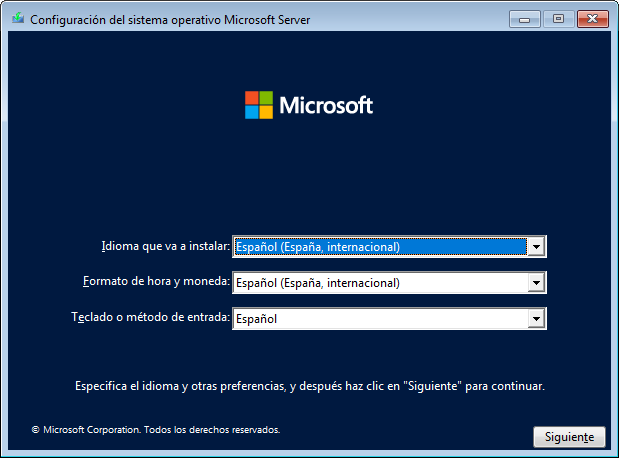
\includegraphics[trim={202 155 203 155},clip,width=\linewidth]{1_instalacion.png}
    \end{minipage}
}

\subsection{Elección del sistema operativo}
Windows Server 2019 tiene distintos modos a la hora de ser instalado, tal como podemos ver en la siguiente captura de pantalla del proceso de instalación:
\begin{center}
  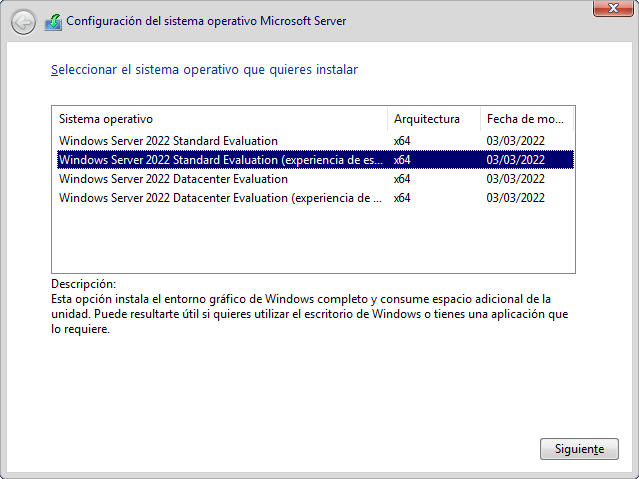
\includegraphics[trim={188 180 195 107},clip,width=10cm]{2_instalacion.png}
\end{center}

Existen dos opciones principales a la hora de elegir, ya que cada una de ellas permitirá instalarlo con o sin experiencia de escritorio. Las opciones principales son:

\begin{itemize}
    \item \textbf{Standard Evaluation}: Útil para empresas medianas o pequeñas, que no requieran de grandes sistemas de virtualización.
    \item \textbf{Datacenter Evaluation}: No habrá límite a la hora de crear máquinas virtuales con un host Hyper-V por cada licencia.
\end{itemize}

Existen más diferencias, y es por eso que Microsoft tiene una página dedicada con la \href{https://docs.microsoft.com/es-es/windows-server/get-started/editions-comparison-windows-server-2019}{comparación de ambas versiones}. Por lo tanto, antes de realizar la instalación para nuestro sistema, debemos realizar una estimación de los requisitos para así poder elegir de manera adecuada.

Nosotros vamos a elegir la versión “Standard Evaluation” con experiencia de escritorio ya que podremos realizar la configuración desde el propio servidor. Dependiendo del caso, habrá que analizar cuál es la mejor opción antes de realizar la instalación.

Al darle a “Siguiente” nos aparecerán los términos de la licencia.

\subsection{Tipo de instalación}
Tras aceptar la licencia nos aparecerá el tipo de instalación que deseamos realizar:
\begin{center}
    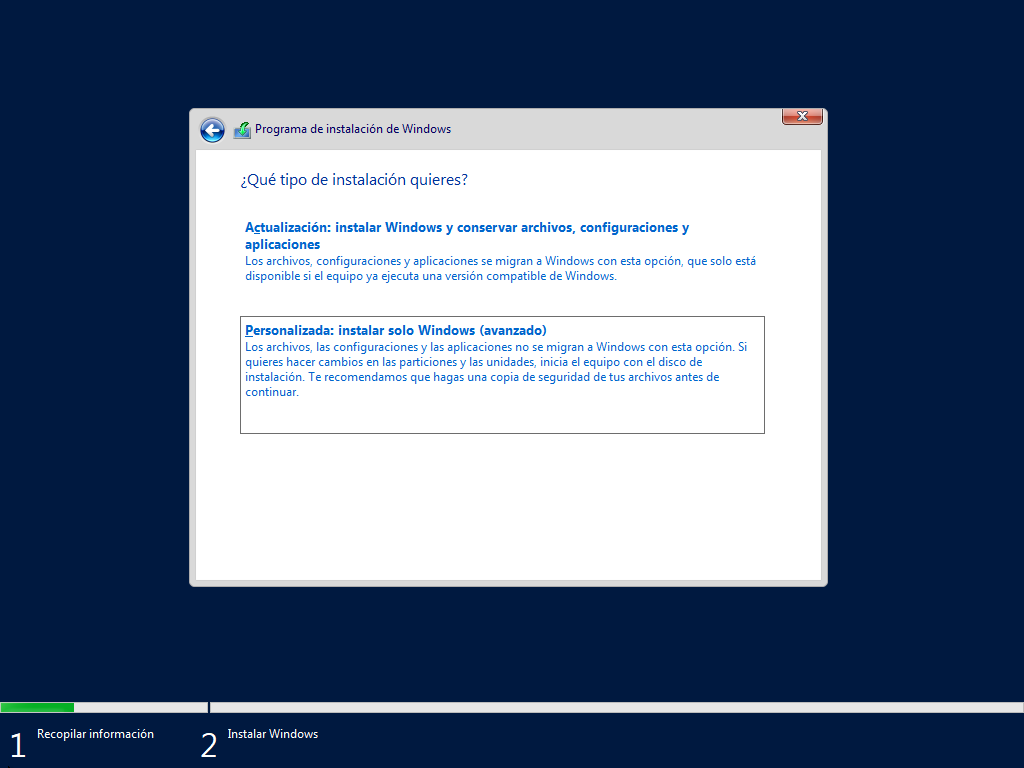
\includegraphics[trim={188 180 195 107},clip,width=10cm]{3_instalacion.png}
\end{center}

\begin{itemize}
    \item \textbf{Actualización}: Para realizar actualizaciones sobre sistemas compatibles ya instalados.
    \item \textbf{Personalizada}: Tal como indica la imagen anterior, los archivos, las configuraciones y las aplicaciones no se migran. En caso de realizar una instalación nueva (como en nuestro caso), \textbf{utilizaremos esta opción}.
\end{itemize}

\subsection{Particionado de discos duros}
Dado que nuestra máquina virtual es nueva, y no tiene ningún sistema operativo previo, vamos a tener que realizar la instalación en el disco duro que se ha añadido a la máquina virtual.

{
    \begin{minipage}{0.6\linewidth}
        \setlength{\parskip}{1.2em}
        Dependiendo del tamaño que hayamos elegido, o incluso los discos duros que tengamos, nos aparecerán en la nueva pantalla del programa de instalación.

        En nuestro caso la máquina virtual cuenta con un único disco duro de 40GB de almacenamiento, en donde realizaremos la instalación de la manera predeterminada que Windows Server elija particionarlo. Por lo tanto, seleccionaremos el disco duro y le daremos al botón de “Siguiente”.
    \end{minipage}
    \hfill
    \begin{minipage}{0.36\linewidth}
        \vspace{-11pt}
        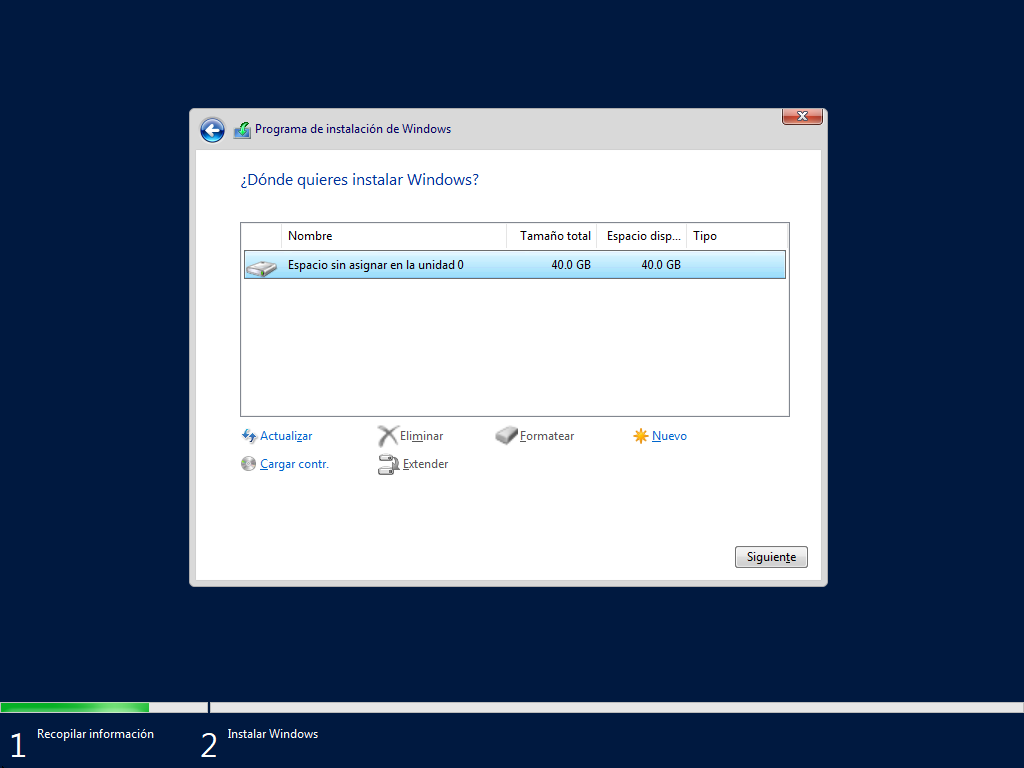
\includegraphics[trim={188 180 195 107},clip,width=\linewidth]{4_instalacion.png}
    \end{minipage}
}

\subsection{Terminar el proceso de instalación}
{
    \begin{minipage}{0.6\linewidth}
        \setlength{\parskip}{1.2em}
        Tras haber seleccionado y haber completado todos los pasos que se han descrito hasta ahora, el proceso de instalación comenzará.

        Este paso de la instalación requerirá de cierto tiempo que dependerá del hardware que tengamos disponible, ya que se realizará la copia de los ficheros de sistema, realizará las instalaciones pertinentes y por último instalará las actualizaciones necesarias.
    \end{minipage}
    \hfill
    \begin{minipage}{0.36\linewidth}
        \vspace{-11pt}
        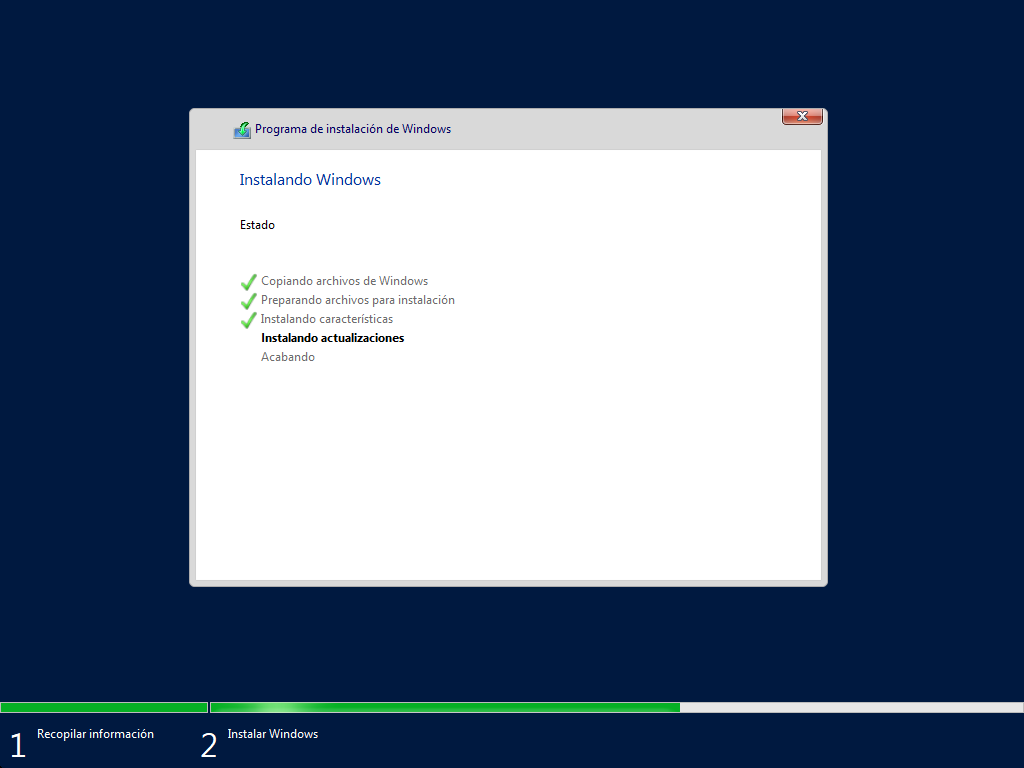
\includegraphics[trim={188 180 195 107},clip,width=\linewidth]{5_instalacion.png}
    \end{minipage}
}

\subsection{Personalizar la configuración}

{
    \begin{minipage}{0.6\linewidth}
        \setlength{\parskip}{1.2em}
        Al terminar el proceso anterior, el último paso nos permitirá realizar la configuración de la contraseña del usuario \textbf{Administrador}.

        Tal como se puede ver a continuación, el nombre de usuario no podrá ser modificado, y nos pedirá la contraseña y la confirmación de la contraseña.
    \end{minipage}
    \hfill
    \begin{minipage}{0.36\linewidth}
        \vspace{-11pt}
        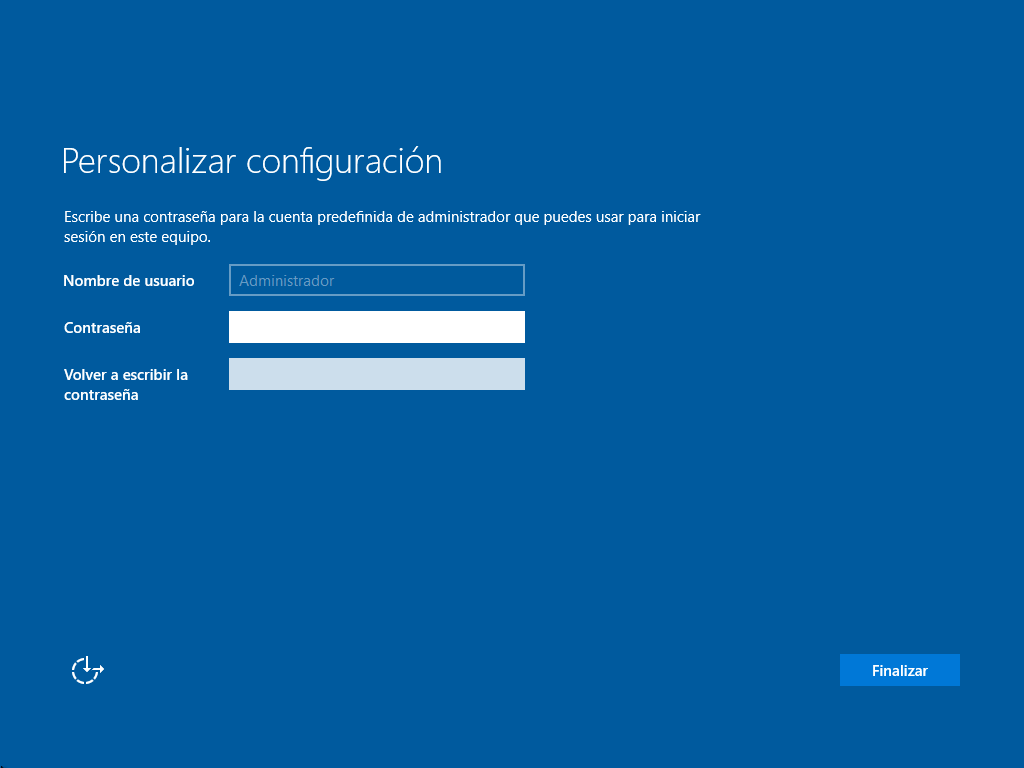
\includegraphics[trim={56 350 300 135},clip,width=\linewidth]{6_instalacion.png}
    \end{minipage}
}

Cabe recordar que esta contraseña es muy importante, ya que con ella realizaremos la configuración de todo el sistema, y por tanto debe ser una contraseña segura y debemos guardarla a buen recaudo. Al darle a “Finalizar” el servidor se reiniciará.

\section{Post-instalación}

Una vez realizada la instalación conviene retirar la imagen ISO del sistema de virtualización, así como incluso retirar el lector DVD virtual, ya que en principio no será necesario volverlo a usar.

Tras el primer arranque nos aparecerá la siguiente pantalla para realizar el login con el usuario Administrador, en donde introduciremos la contraseña que hemos puesto en el paso anterior. Una vez introducida, la siguiente pantalla será la pantalla de inicio donde podremos ver el panel de administrador del servidor.

\begin{tcolorbox}[title=Windows Server 2019 recién instalado,colback=white]
    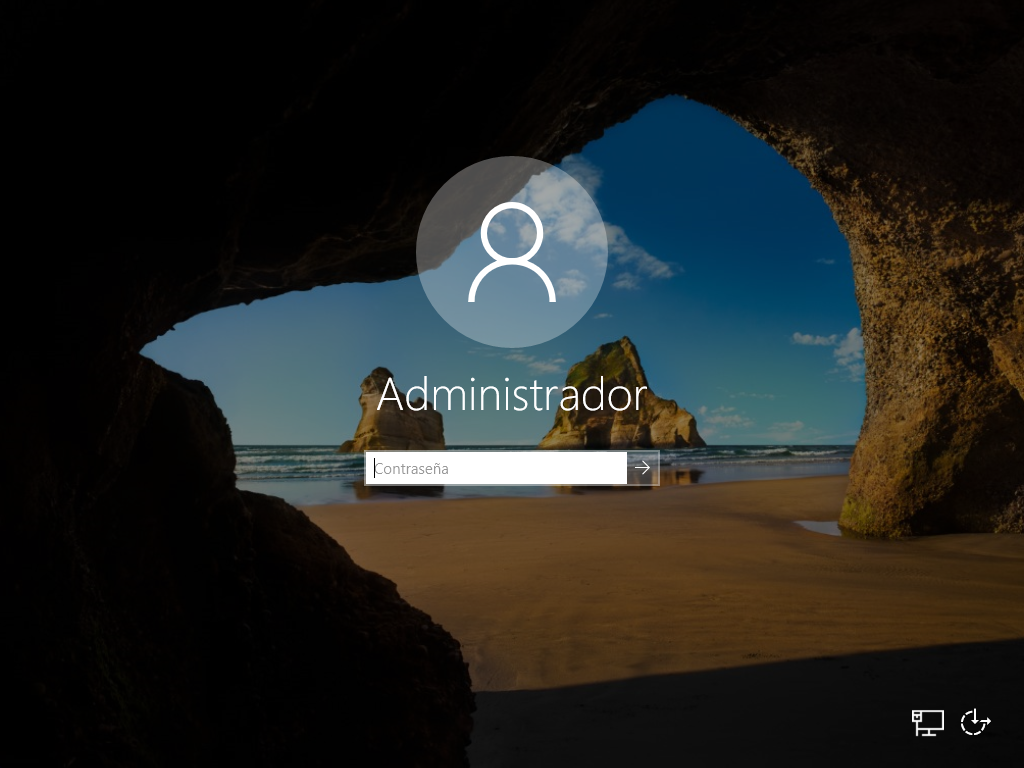
\includegraphics[width=0.48\linewidth]{7_instalacion.png}
    \hfill
    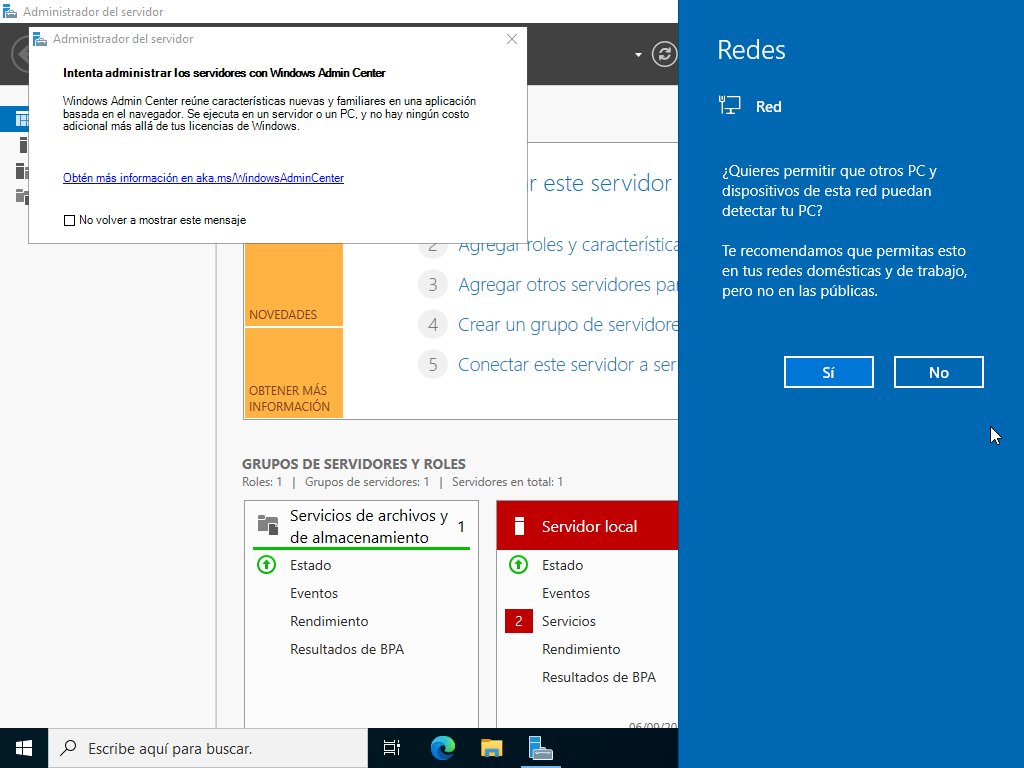
\includegraphics[width=0.48\linewidth]{8_instalacion.png}
\end{tcolorbox}


\chapter{Windows Server 2019 como servidor de red}
Windows Server 2019 tras la instalación no es más que un sistema operativo “normal”, que potencialmente se puede convertir en un Sistema Operativo de red, con funcionalidad para administrar usuarios, creación de grupos, permisos, … Para realizar estas funciones debemos de configurar el Sistema Operativo.

Como se ha observado, durante la instalación del Sistema Operativo apenas se realizan preguntas, por lo que es el propio instalador el que ha tomado ciertas decisiones por nosotros, como son:

\begin{itemize}
    \item Obtención de IP (a través de DHCP o Dynamic Host Configuration Protocol)
    \item Nombre del equipo
\end{itemize}

Estos datos los modificaremos más adelante.


\section{Entendiendo conceptos en Windows Server}
Durante la instalación y promoción del servidor como controlador de dominio y configuración de Active Directory, existen ciertos conceptos que son intrínsecos a cómo va a funcionar Windows Server como servidor  y que deben de ser entendidos.


\subsection{Active Directory}
\textbf{\textit{Active Directory}} (AD), o \textbf{Directorio Activo}, son los términos que utiliza Microsoft para referirse a su implementación de servicio de directorio en una red distribuida de computadores. Utiliza distintos protocolos, principalmente \href{https://es.wikipedia.org/wiki/Protocolo_ligero_de_acceso_a_directorios}{LDAP}, \href{https://es.wikipedia.org/wiki/Sistema_de_nombres_de_dominio}{DNS}, \href{https://es.wikipedia.org/wiki/Protocolo_de_configuraci%C3%B3n_din%C3%A1mica_de_host}{HDCP} y \href{https://es.wikipedia.org/wiki/Kerberos}{Kerberos}.

De forma sencilla se puede decir que es un servicio establecido en uno o varios servidores en donde se crean objetos tales como usuarios, equipos o grupos, con el objetivo de administrar los inicios de sesión en los equipos conectados a la red, así como también la administración de políticas en toda la red.

Su estructura jerárquica permite mantener una serie de objetos relacionados con componentes de una red, como usuarios, grupos de usuarios, permisos y asignación de recursos y políticas de acceso. (Fuente: \href{https://es.wikipedia.org/wiki/Active_Directory}{wikipedia}).


\subsection{Dominio}
Un dominio es una colección de objetos dentro del directorio que forman un subconjunto administrativo. Pueden existir diferentes dominios dentro de un bosque, cada uno de ellos con su propia colección de objetos y unidades organizativas.

Para poner nombre a los dominios se utiliza el protocolo DNS. Por este motivo, Active Directory necesita al menos un servidor DNS instalado en la red

\subsection{Unidad Organizativa (UO)}
En inglés Organizational Unit (OU). Es la unidad jerárquica inferior al dominio que puede tener objetos y/u otras UO. Más adelante las usaremos para la creación de GPOs.

\infobox{\textbf{Las Unidades Organizativas (UO) son contenedores dentro del Active Directory}}


\subsection{Objeto}
La palabra Objeto se utiliza como nombre genérico para referirnos a cualquiera de los componentes que forman parte del directorio, como una impresora o una carpeta compartida, pero también un usuario, un grupo, etc. Incluso podemos utilizar la palabra objeto para referirnos a una Unidad organizativa.

Cada objeto dispondrá de una serie de características específicas (según la clase a la que pertenezca) y un nombre que permitirá identificarlo de forma precisa. En general, los objetos se organizan en tres categorías:
\begin{itemize}
    \item \textbf{Usuarios}: identificados a través de un nombre (y, casi siempre, una contraseña), que pueden organizarse en grupos, para simplificar la administración.
    \item \textbf{Recursos}: que son los diferentes elementos a los que pueden acceder, o no, los usuarios según sus privilegios. Por ejemplo, carpetas compartidas, impresoras, etc.
    \item \textbf{Servicios}: que son las diferentes funciones a las que los usuarios pueden tener acceso. Por ejemplo, el correo electrónico.
\end{itemize}


\subsection{Controlador de dominio}
Un Controlador de Dominio (domain controller) contiene la base de datos de objetos del directorio para un determinado dominio, incluida la información relativa a la seguridad. Además, será responsable de la autenticación de objetos dentro de su ámbito de control.

En un dominio dado, puede haber varios controladores de dominio asociados, de modo que cada uno de ellos represente un rol diferente dentro del directorio. Sin embargo, a todos los efectos, todos los controladores de dominio, dentro del mismo dominio, tendrán la misma importancia.


\subsection{Árbol}
Un Árbol es simplemente una colección de dominios que dependen de una raíz común y se encuentran organizados como una determinada jerarquía. Dicha jerarquía también quedará representada por un espacio de nombres DNS común.

De esta forma, sabremos que los dominios \textbf{mikeldi.com} e \textbf{informatica.mikeldi.com} forman parte del mismo árbol, mientras que \textbf{mikeldi.com} y \textbf{linux.org} no.

Si un determinado usuario es creado dentro de un dominio, éste será reconocido automáticamente en todos los dominios que dependan jerárquicamente del dominio al que pertenece.


\subsection{Bosque}
El Bosque es el mayor contenedor lógico dentro de Active Directory, abarcando a todos los dominios dentro de su ámbito. Los dominios están interconectados por Relaciones de confianza transitivas que se construyen automáticamente (consultar más adelante el concepto de Relación de confianza). De esta forma, todos los dominios de un bosque confían automáticamente unos en otros y los diferentes árboles podrán compartir sus recursos.

\begin{center}
    \vspace{-15pt}
    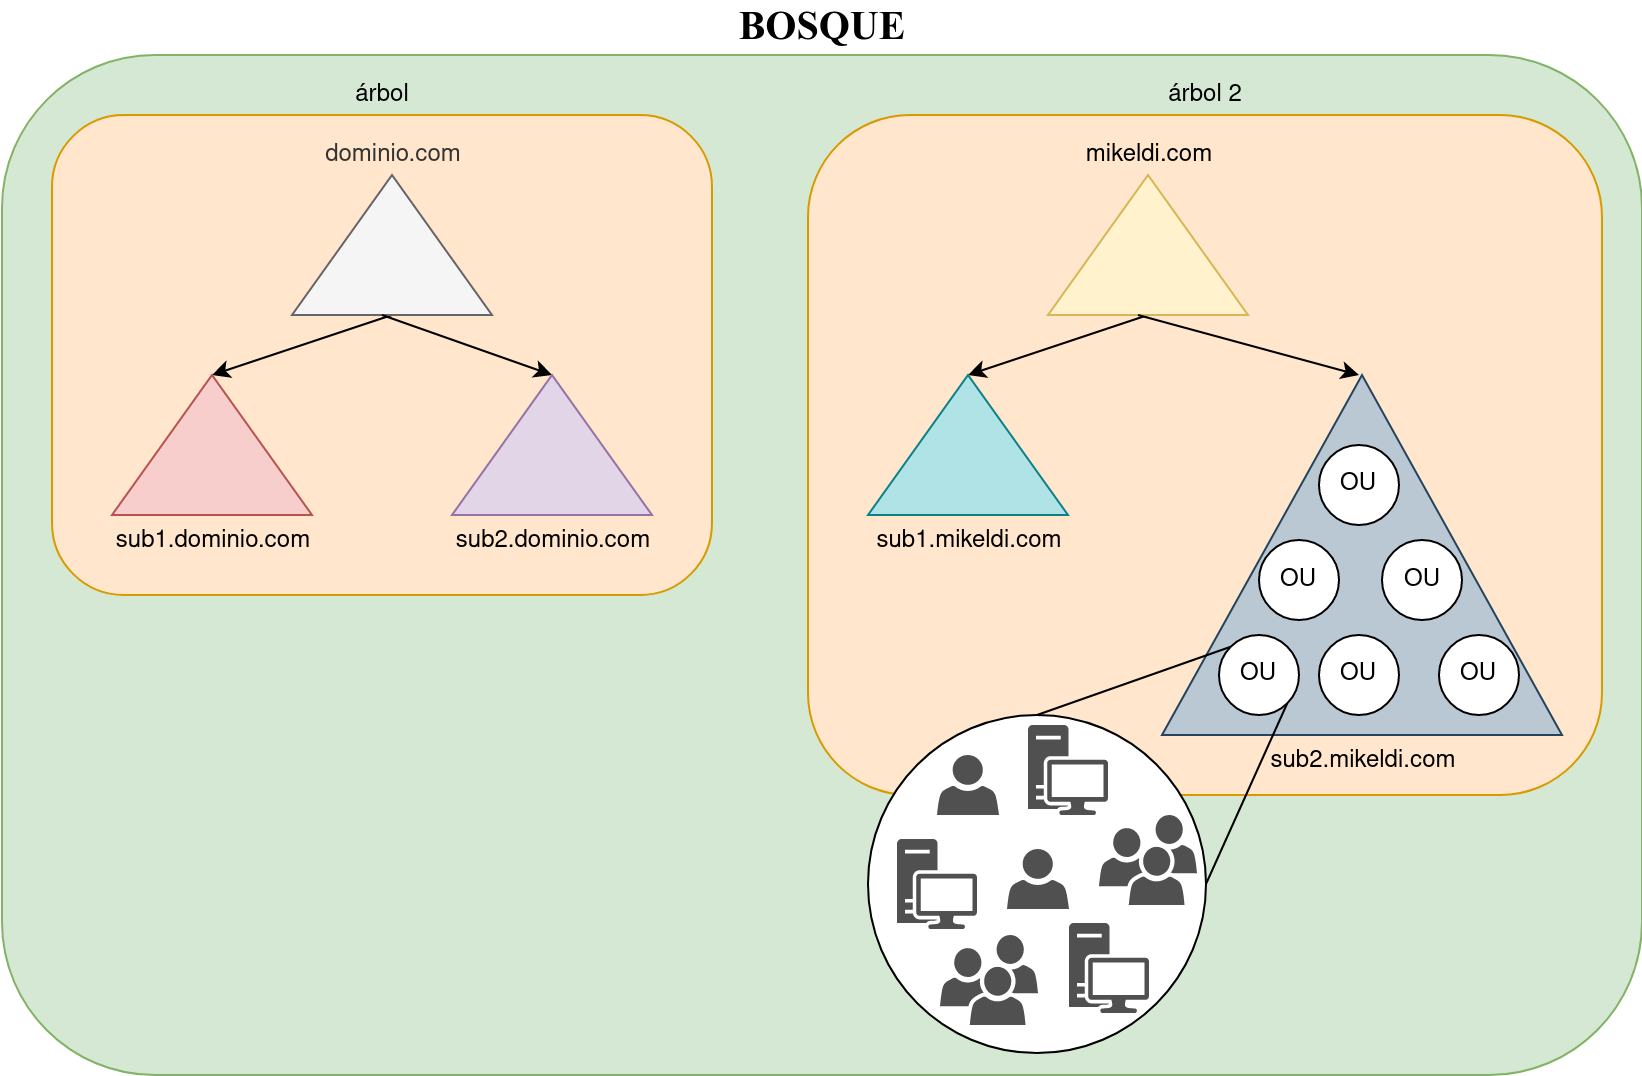
\includegraphics[width=0.6\linewidth]{bosque_directorio_activo.png}
    \vspace{-15pt}
\end{center}

Como ya hemos dicho, los dominios pueden estar organizados jerárquicamente en un árbol que comparte un espacio de nombres DNS común. A su vez, \textbf{diferentes árboles pueden estar integrados en un bosque}. Al tratarse de \textbf{árboles diferentes, no compartirán el mismo espacio de nombres}.

\subsection{Relaciones de confianza}
En el contexto de Active Directory, las Relaciones de confianza son un método de comunicación seguro entre dominios, árboles y bosques. Las relaciones de confianza permiten a los usuarios de un dominio del Directorio Activo autenticarse en otro dominio del directorio.


\section{Configurando Windows Server como servidor en Red}
Antes de promocionar el servidor a controlador de dominio, y por tanto convertirlo en un servidor en red, debemos realizar unos pasos previos de configuración. Los pasos que tendremos que realizar serán los siguientes:

\begin{itemize}
    \item Configurar una \textbf{IP estática} al equipo: Todos los servidores en una red (tanto pública como privada) debe de tener una IP estática en la misma. Deberemos de conocer el direccionamiento de la red, y confirmar que la IP que vamos a configurar no está siendo utilizada por otro equipo.
    \begin{itemize}
        \item El cambio de IP se realiza en “\textbf{Configuración de Red e Internet}”, en este caso “Protocolo de Internet versión 4” y poniendo la IP correspondiente a nuestra red.
        \begin{center}
            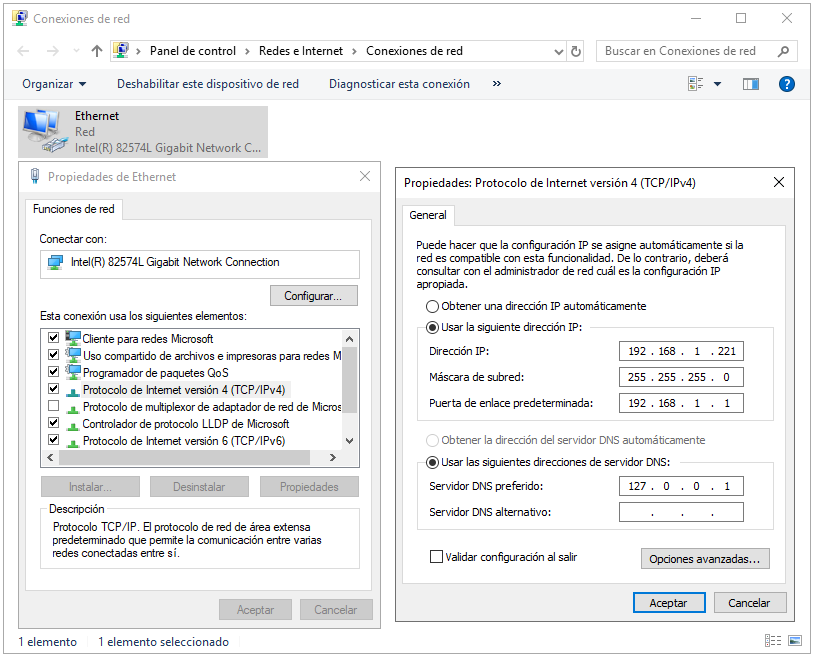
\includegraphics[trim={245 105 540 139},clip,width=0.8\linewidth]{cambiar_ip_windows.png}
        \end{center}
        \item También vamos a configurar como \textbf{Servidor DNS preferido} la IP localhost, “127.0.0.1”, para que posteriormente Active Directory ejerza de DNS local.
    \end{itemize}

    \item Cambiar el \textbf{nombre del equipo}: Para que los servidores sean fácilmente identificables, debemos proporcionarles un nombre de equipo que indique cuáles son sus funciones. En nuestro caso, podemos llamarlo “\textbf{AD}” (de Active Directory) o “\textbf{DC}” (de \textit{Domain Controller}). Tras realizar el cambio, el servidor deberá reiniciarse. El cambio se puede realizar desde varias partes de Windows Server, como por ejemplo:
    \begin{itemize}
        \item Click derecho en Inicio → Sistema
        \item Panel de control → Sistema y Seguridad → Sistema → Cambiar Configuración
    \end{itemize}
    \begin{center}
        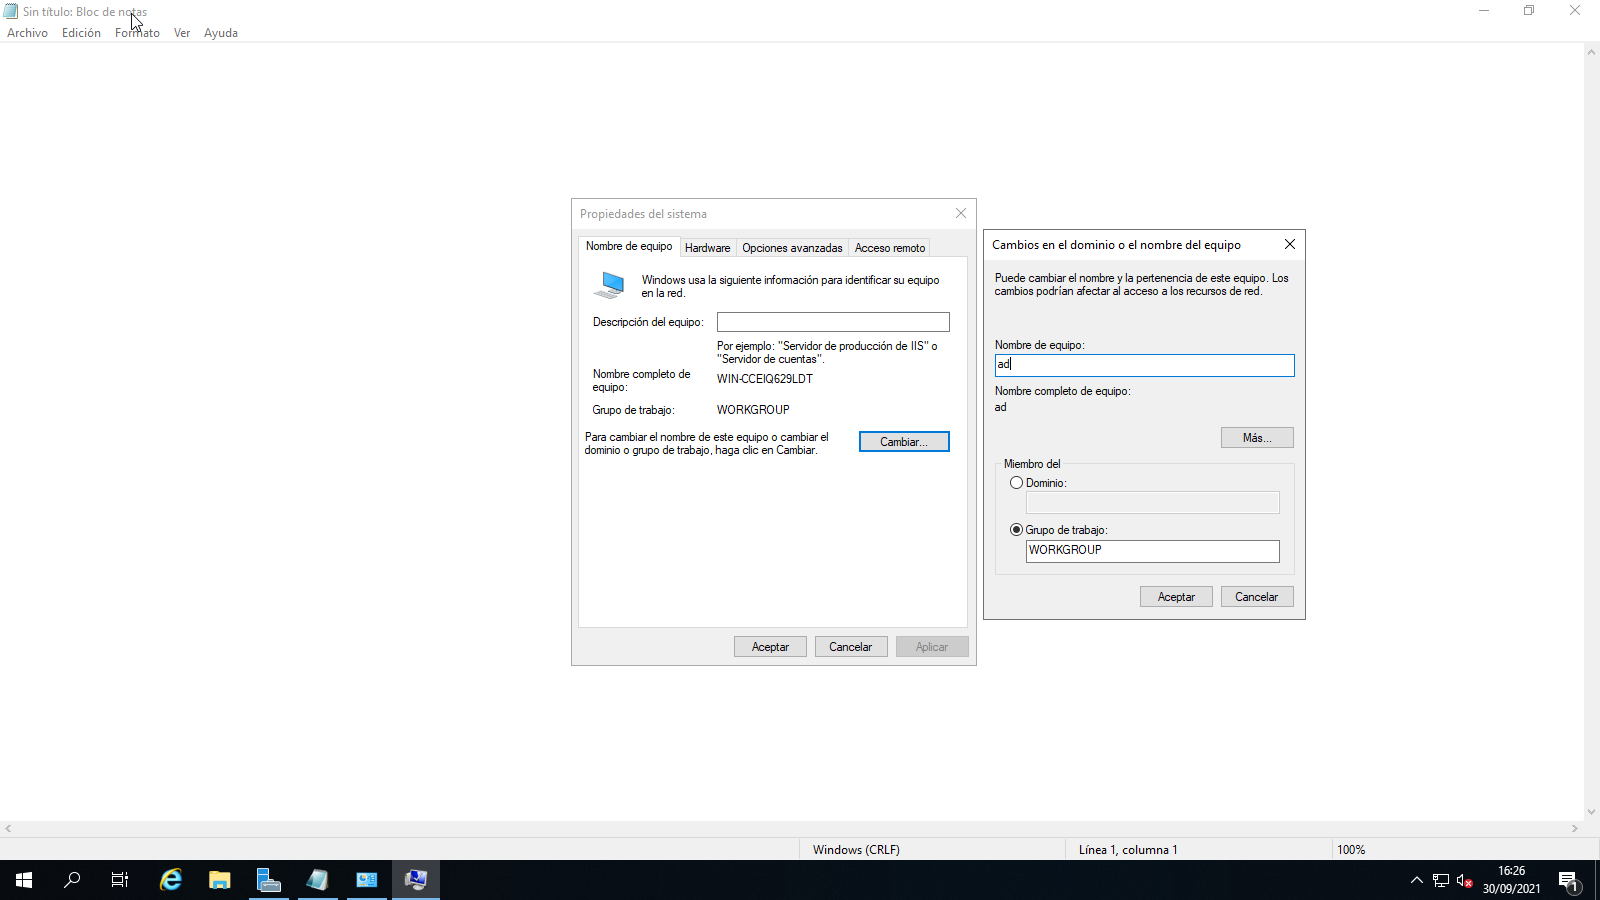
\includegraphics[trim={568 230 290  195},clip,width=0.8\linewidth]{cambiar_nombre_windows.png}
    \end{center}

    \item Asegurar que la zona horaria es la adecuada
    \begin{itemize}
        \item Comprobar servicio de hora
        \item Comprobar que la actualización de la hora es automática
    \end{itemize}

\end{itemize}


\section{Instalar Active Directory}
Para promocionar el servidor a controlador de dominio de Active Directory debemos de realizar la instalación del rol. Para ello, iremos al “\textbf{Administrador del Servidor}”.

\begin{tcolorbox}[title=Panel del Administrador del servidor]
    \begin{center}
        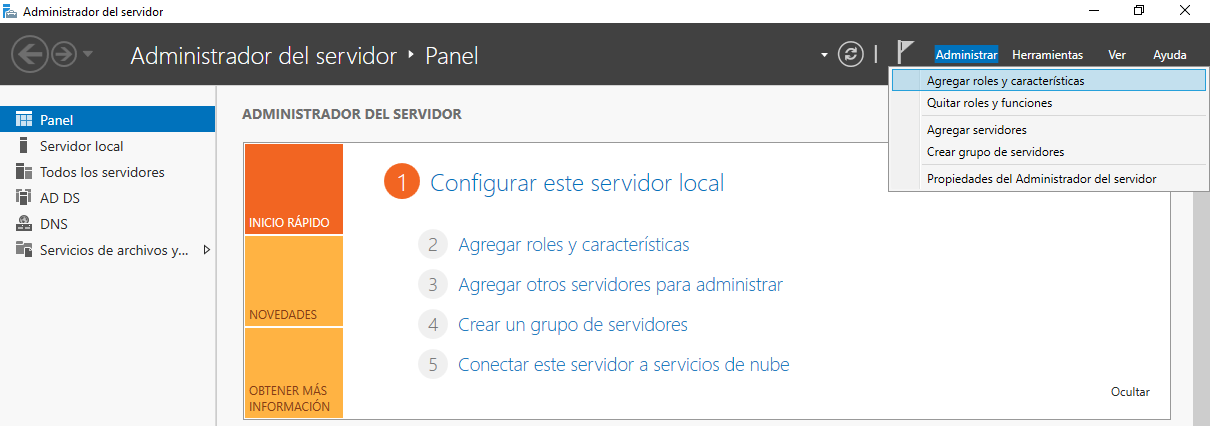
\includegraphics[width=0.8\linewidth]{administrador_del_servidor.png}
    \end{center}
\end{tcolorbox}

aremos click en “Administrar”, “Agregar roles y características” y nos saldrá una nueva ventana, con un aviso del asistente y al darle a “Siguiente”, elegiremos la primera opción, “\textbf{Instalación basada en características y roles}” y volveremos a darle a “Siguiente” en el asistente: